\section{Longitudinal Connectivity {
\includegraphics[height=15pt]{connectivity-x-small}}}

\subsection{Reservoir Sedimentation - Principles}


\subsection{Mountain River Engineering}
\begin{frame}{\secname\vspace{0.1cm}\\\textcolor{anthrazit!80!white}{\subsecname}}
	\begin{tikzpicture}
		\clip (0,0) rectangle (\paperwidth,\paperheight);
		\onslide<1->{
		\begin{scope}
				\node[anchor=south west, xshift=0.0\paperwidth, yshift=0.31\paperheight] {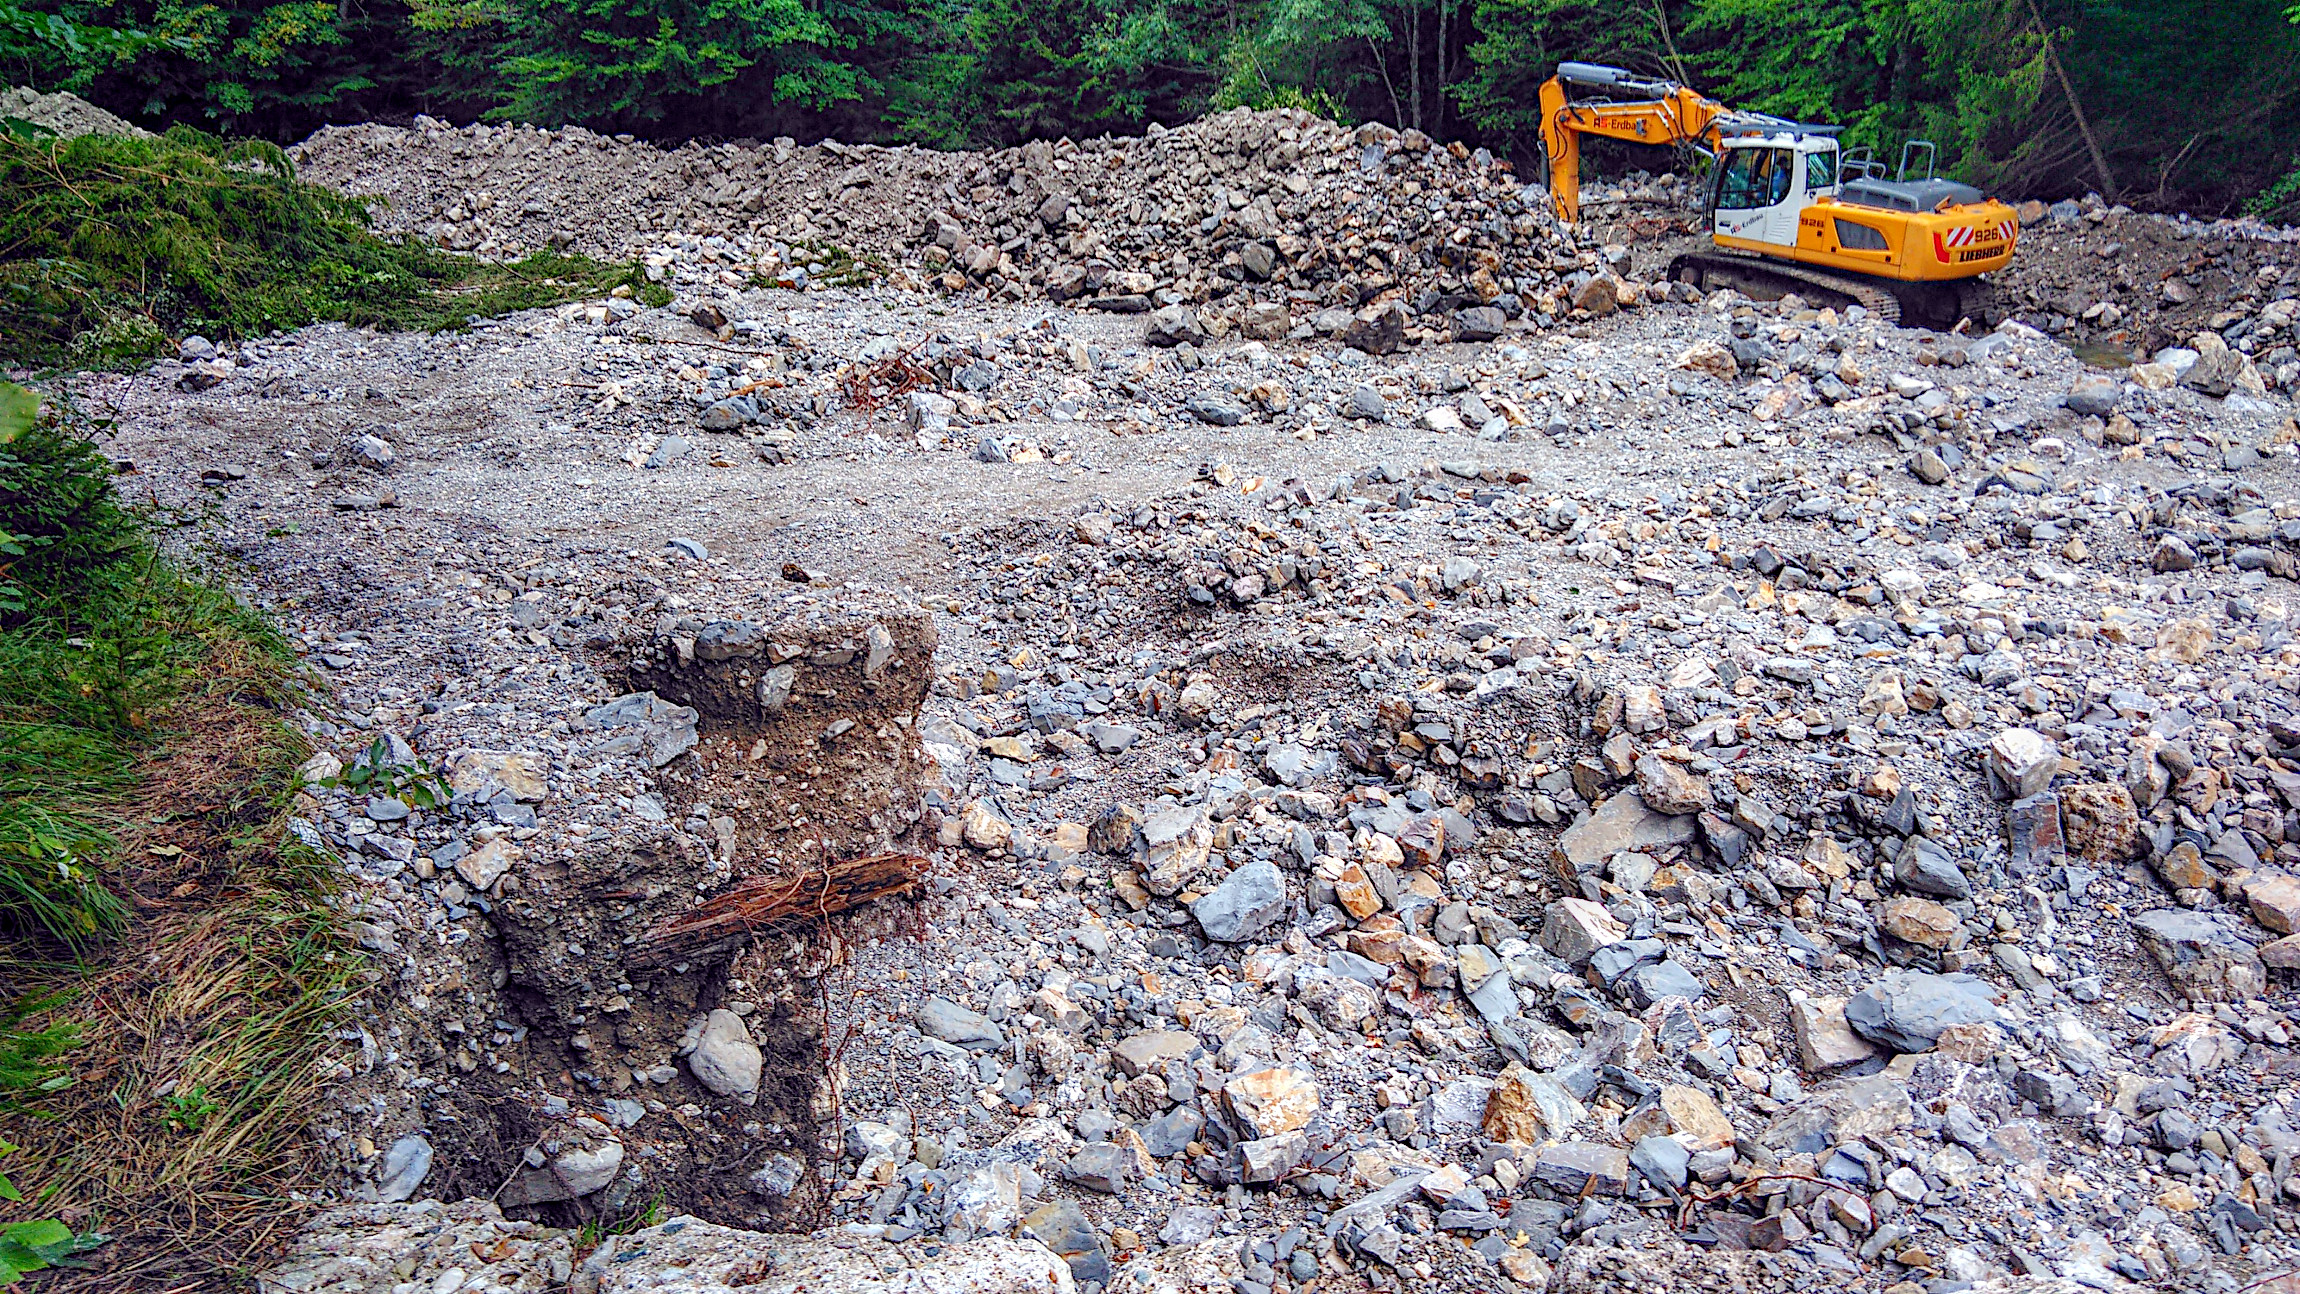
\includegraphics[width=0.865\paperwidth]{jenbach-bagger}};
		\end{scope}}
		\node[anchor=south west, xshift=0.33\paperwidth, yshift=2.13cm, text=black, text width=0.5\paperwidth,align=left]{\tiny \textcolor{gray}{Jenbach, Bavarian Alps}};
	\end{tikzpicture}
\end{frame}
\begin{frame}{\secname\vspace{0.1cm}\\\textcolor{anthrazit!80!white}{\subsecname}}
	\begin{tikzpicture}
		\clip (0,0) rectangle (\paperwidth,\paperheight);
		\onslide<1->{
			\begin{scope}
				\node[anchor=south west, xshift=0.0\paperwidth, yshift=0.31\paperheight] {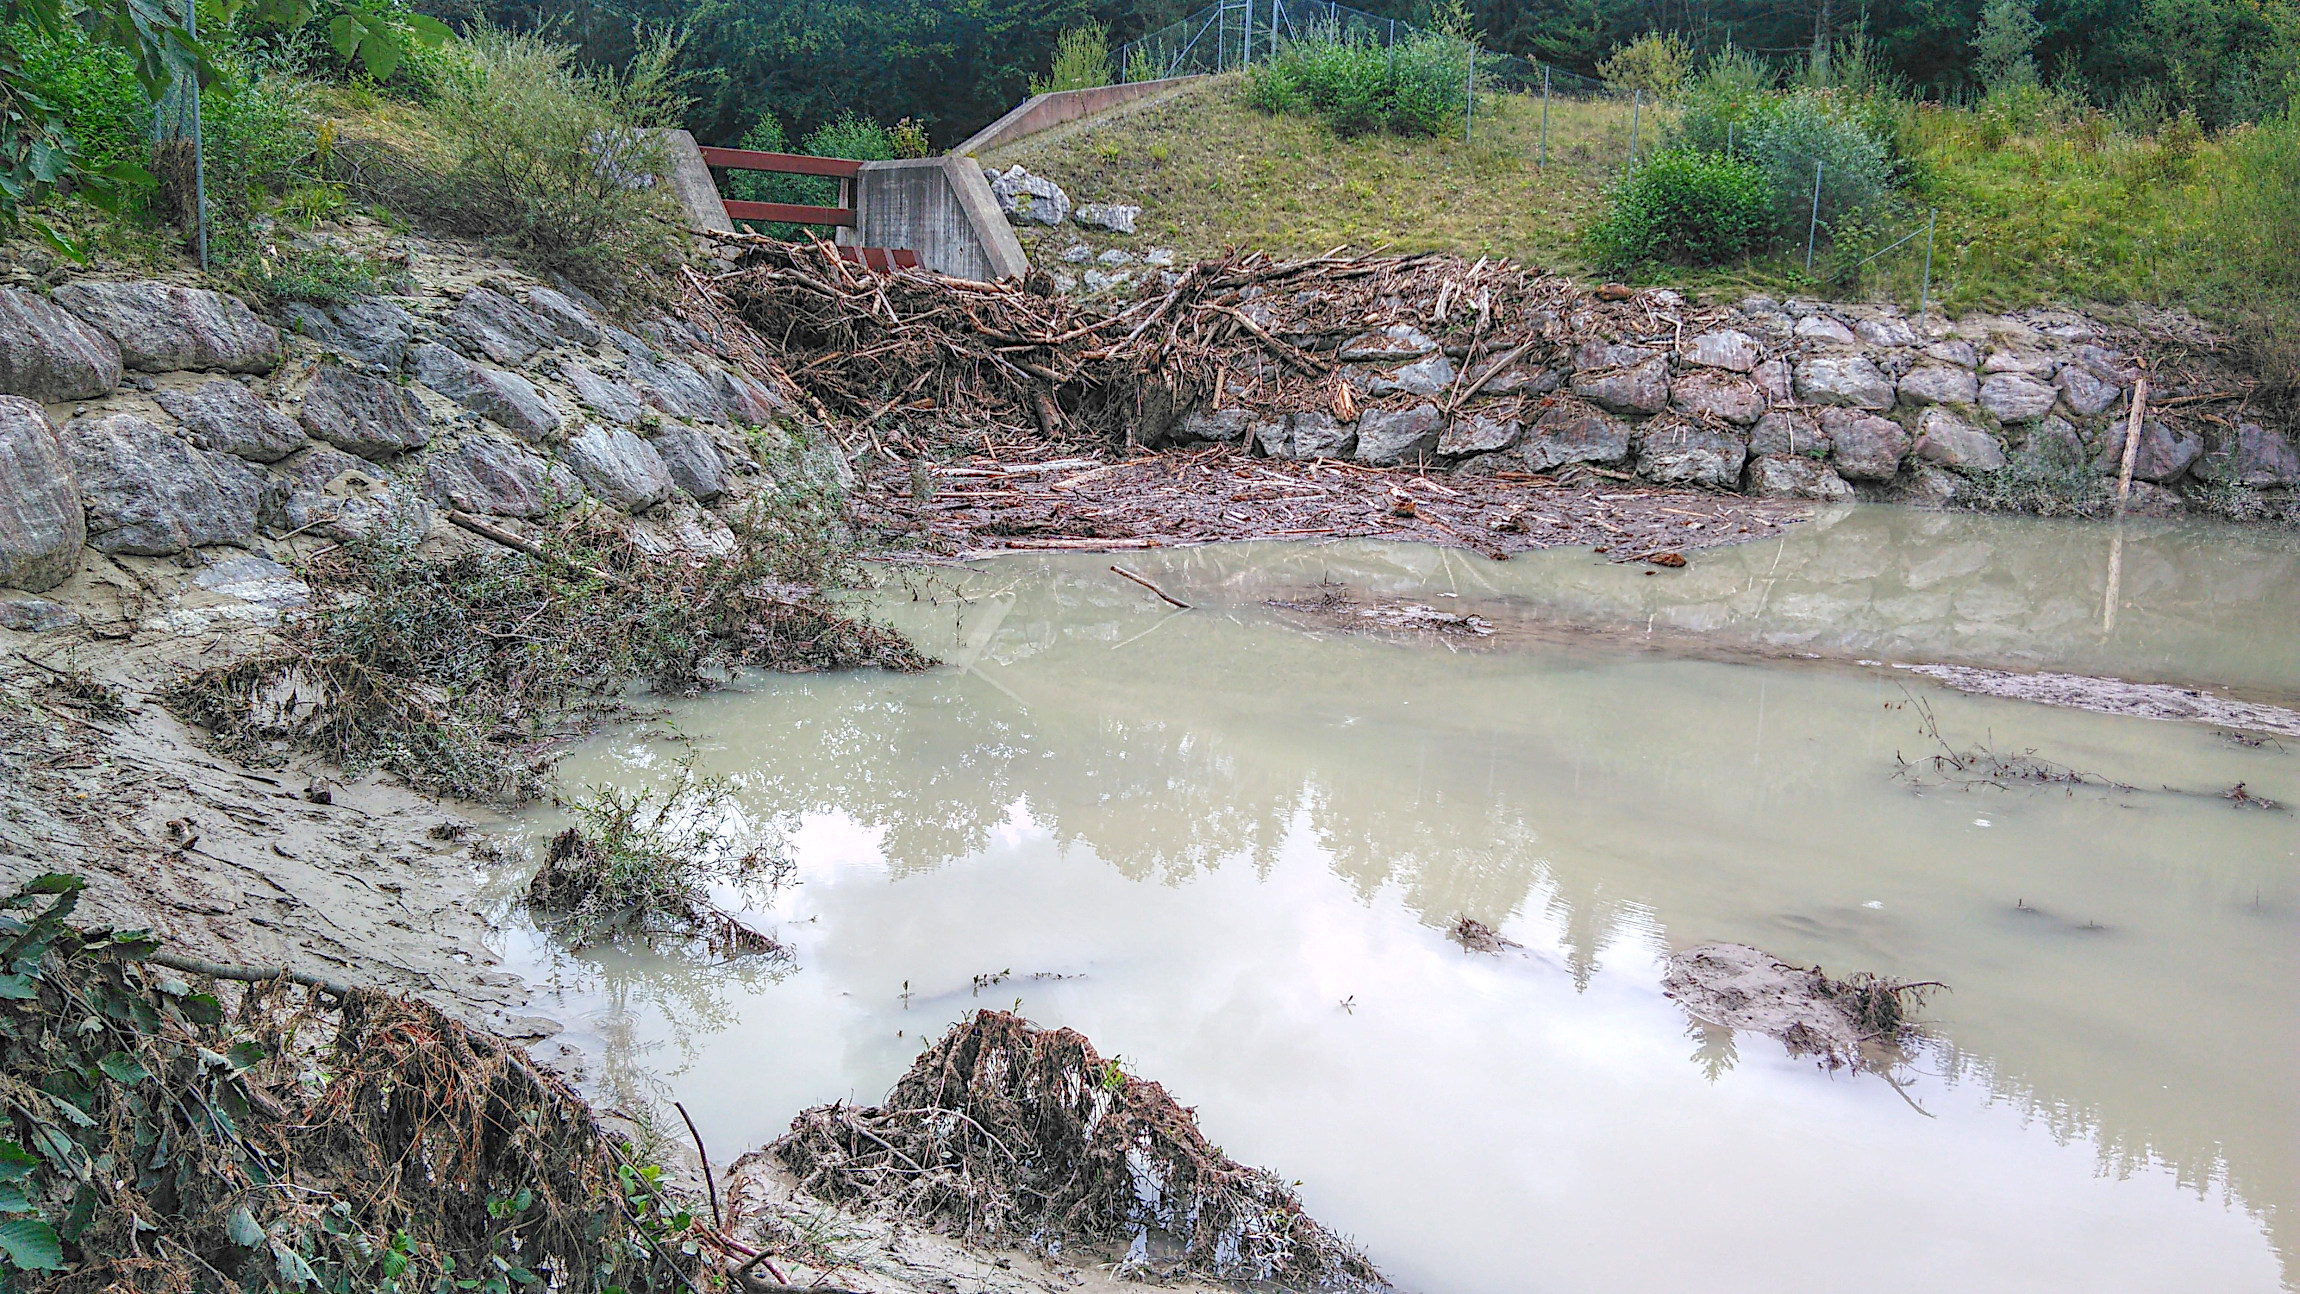
\includegraphics[width=0.865\paperwidth]{jenbach-trap-filled}};
		\end{scope}}
	\node[anchor=south west, xshift=0.33\paperwidth, yshift=2.13cm, text=black, text width=0.5\paperwidth,align=left]{\tiny \textcolor{gray}{Sediment trap at the Jenbach, Bavarian Alps}};
	\end{tikzpicture}
\end{frame}



\begin{frame}{\secname\vspace{0.1cm}\\\textcolor{anthrazit!80!white}{\subsecname}}
	\begin{tikzpicture}
		\clip (0,0) rectangle (\paperwidth,\paperheight);
		\onslide<1->{
			\begin{scope}
				\node[anchor=south west, xshift=0.0\paperwidth, yshift=0.34\paperheight] {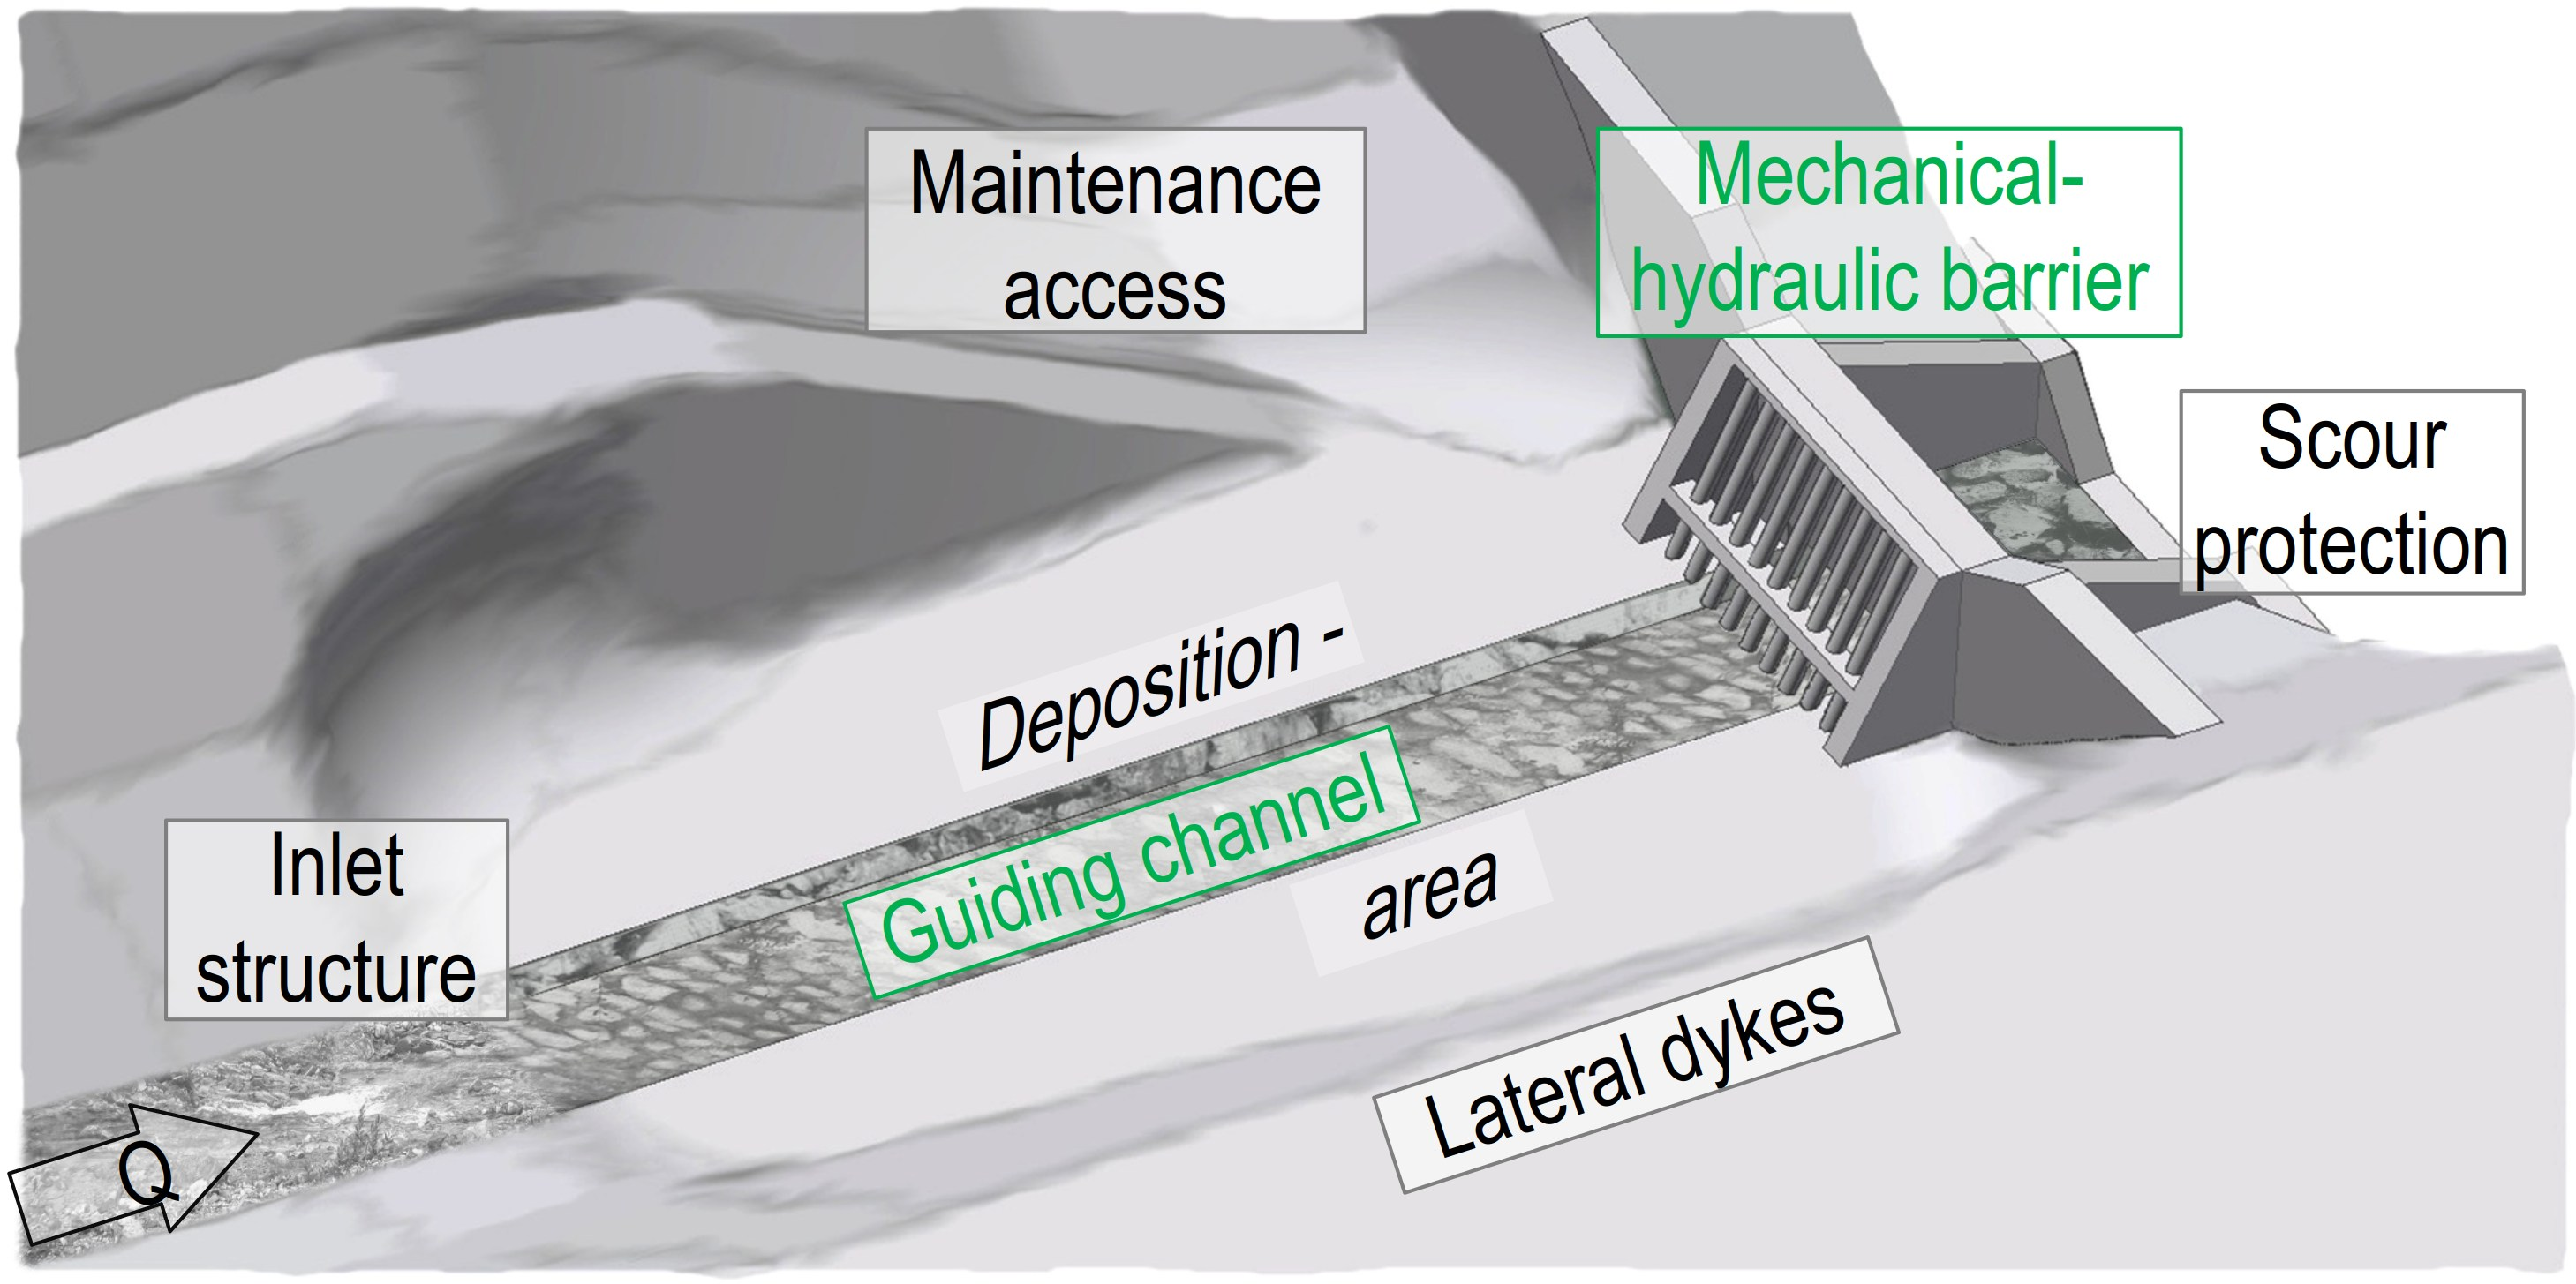
\includegraphics[width=0.88	\paperwidth]{check-dam-concept}};
		\end{scope}}
		\onslide<1-1>{
			\node[anchor=south west, xshift=0.21\paperwidth, yshift=2.21cm, text=black, text width=0.55\paperwidth,align=left]{\tiny \textcolor{gray}{Source: \sscURL{Schwindt \textit{et al.} (2018)}{https://www.nat-hazards-earth-syst-sci.net/18/647/2018/} / \sscURL{Moldenhauer, Piton, Schwindt \textit{et al. (2021)}}{https://www.sciencedirect.com/science/article/pii/S1001627920300792}}};}
	\end{tikzpicture}
\end{frame}

\subsection{Sediment Management in Reservoirs}

\begin{frame}{\secname\vspace{0.1cm}\\\textcolor{anthrazit!80!white}{\subsecname}}
	\begin{tikzpicture}
		\clip (0,0) rectangle (\paperwidth,\paperheight);
		\onslide<1->{
			\begin{scope}
				\node[anchor=south west, xshift=0.0\paperwidth, yshift=0.48\paperheight] {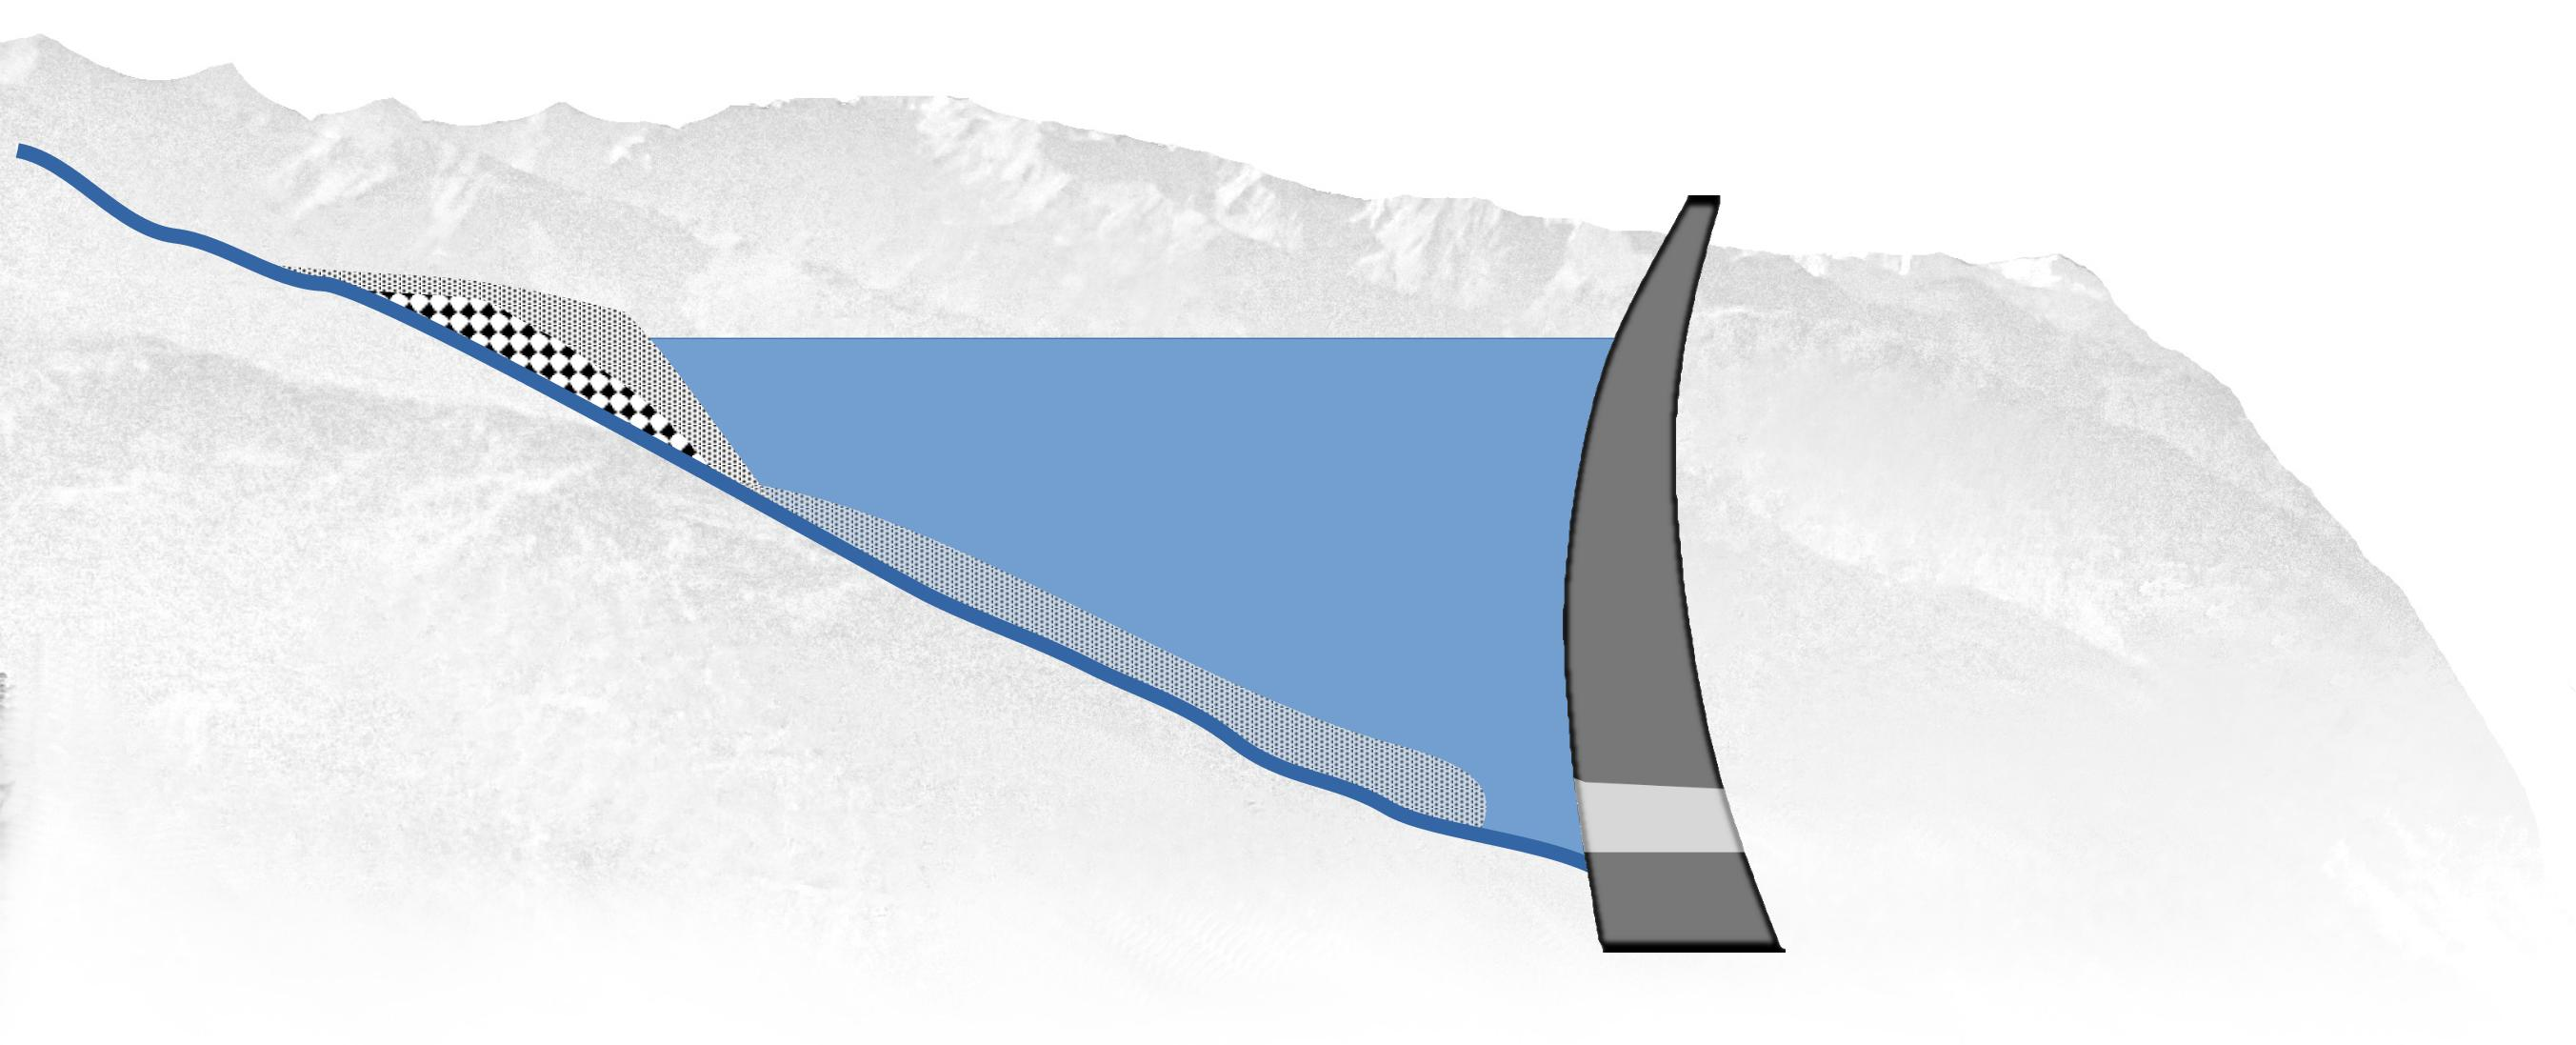
\includegraphics[width=0.91\paperwidth]{dam-scheme-zoom}};
		\end{scope}}
%		\onslide<2->{
%			\begin{scope}
%				\node[anchor=south west, xshift=0.0\paperwidth, yshift=0.48\paperheight] {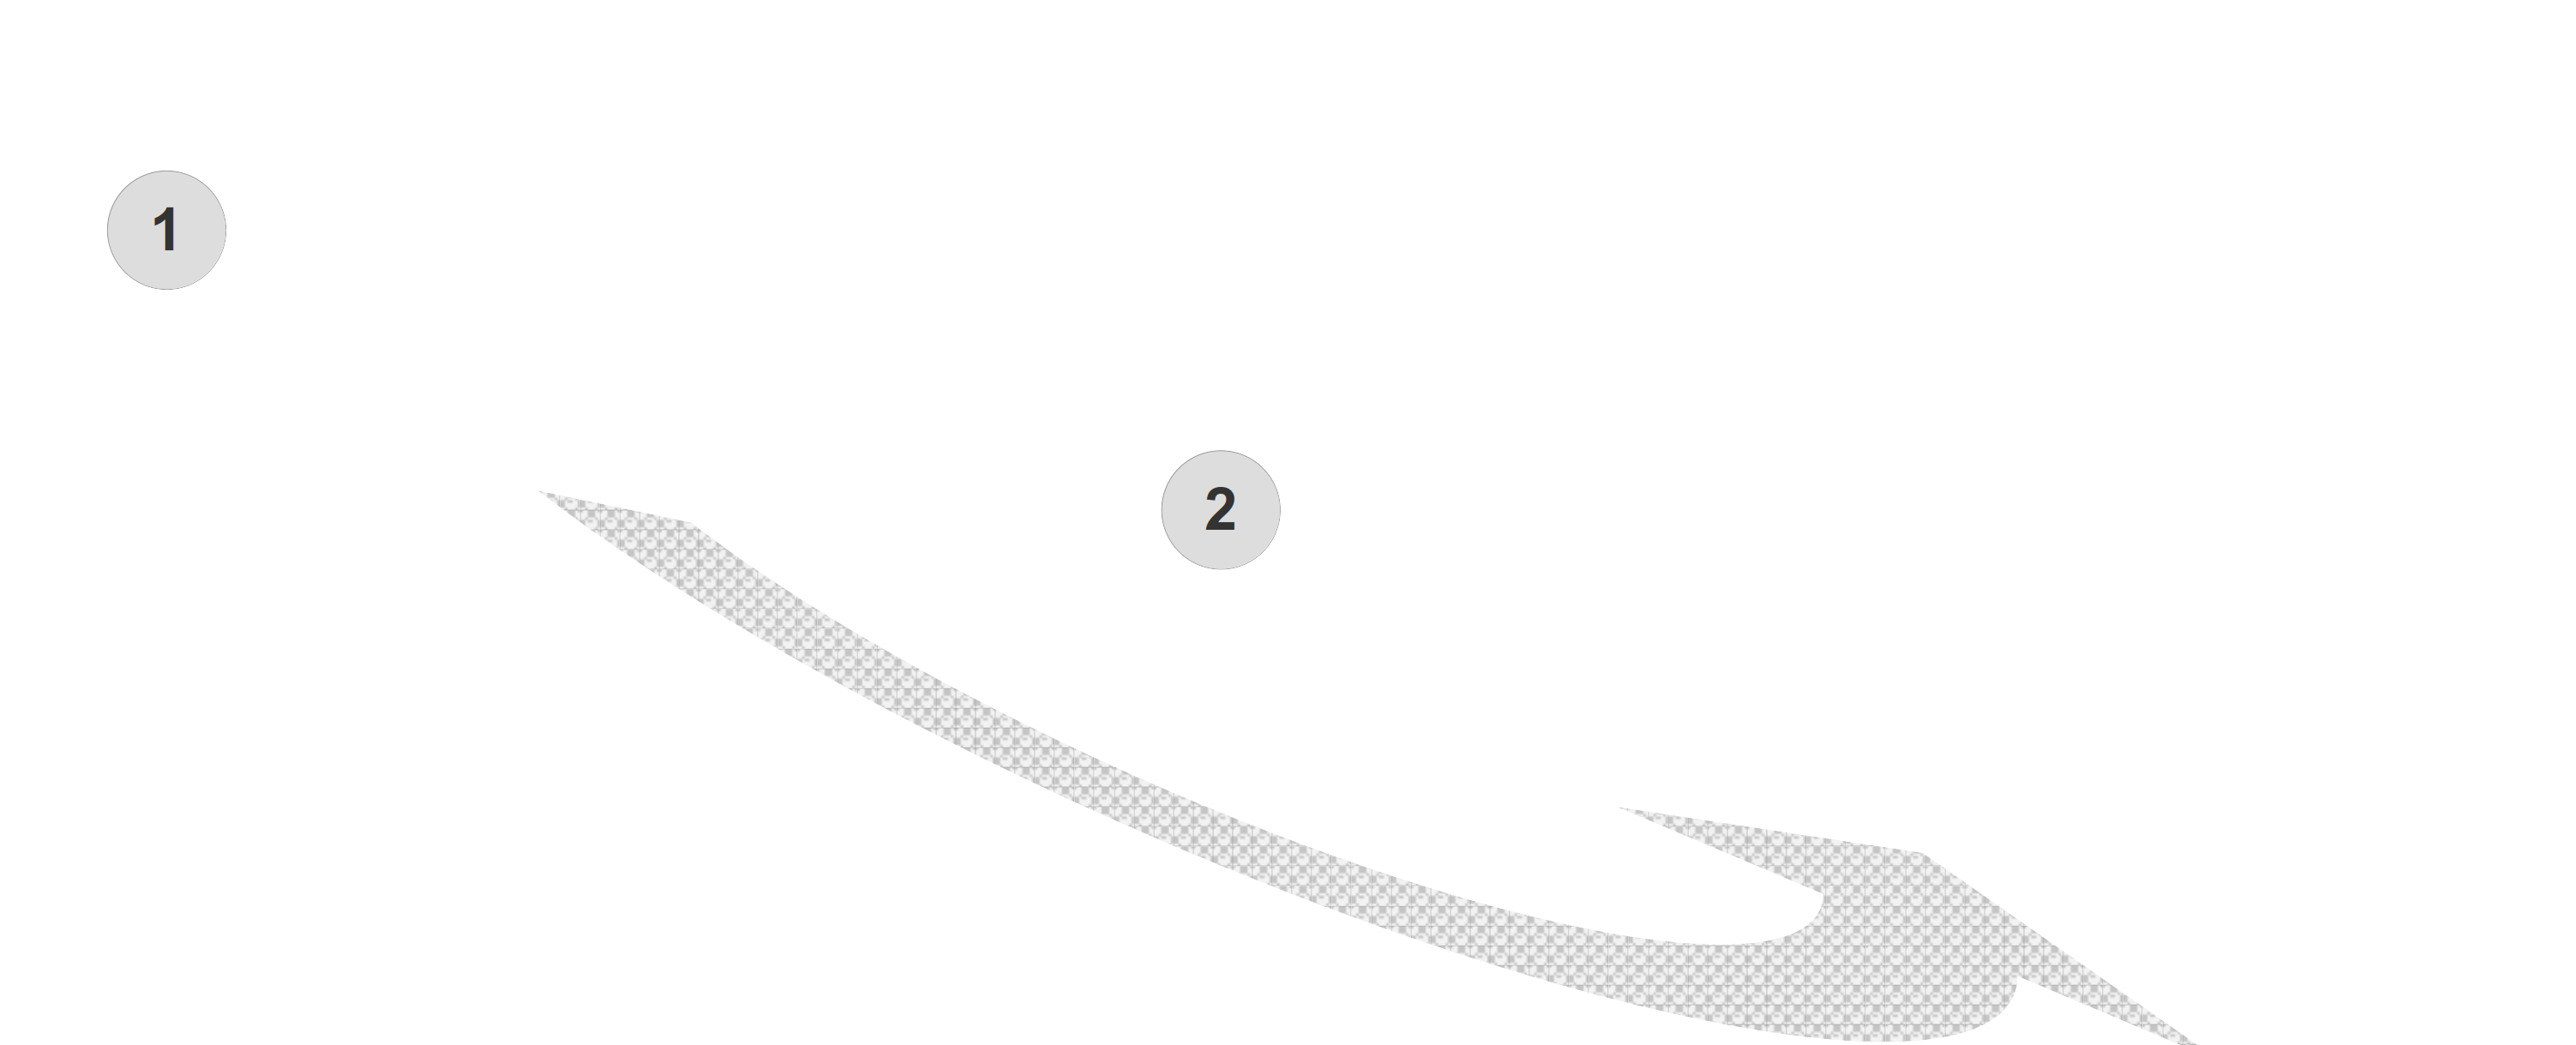
\includegraphics[width=0.91\paperwidth]{dam-scheme-zoom-overlay}};
%		\end{scope}}
		\onslide<1->{
			\begin{scope}
				\node[anchor=south west, xshift=0.0\paperwidth, yshift=0.32\paperheight] {
					\begin{minipage}{0.95\textwidth}
						\begin{itemize}
							% \setlength\itemsep{0.7em}
							\item[\faHandORight]\ Coarse \& fine sediment deposits in delta regions (reservoir head)
							\item[\faHandORight]\ Very fine, partially cohesive sediment disperses in the entire reservoir
							\item[\faHandORight]\ Turbidity currents move suspended sediment close to dams
						\end{itemize}
					\end{minipage}
				};
		\end{scope}}
		\onslide<1->{
			\node[anchor=south west, xshift=0.33\paperwidth, yshift=2.1947cm, text=black, text width=0.5\paperwidth,align=left]{\tiny \textcolor{gray}{Image concept from Chamoun \textit{et al.} (2017) / SCCER-SoE}};}
	\end{tikzpicture}
\end{frame}

\begin{frame}{\secname\vspace{0.1cm}\\\textcolor{anthrazit!80!white}{\subsecname}}
	\begin{tikzpicture}
		\clip (0,0) rectangle (\paperwidth,\paperheight);
		\onslide<1->{
			\begin{scope}
				\node[anchor=south west, xshift=0.06\paperwidth, yshift=0.27\paperheight] {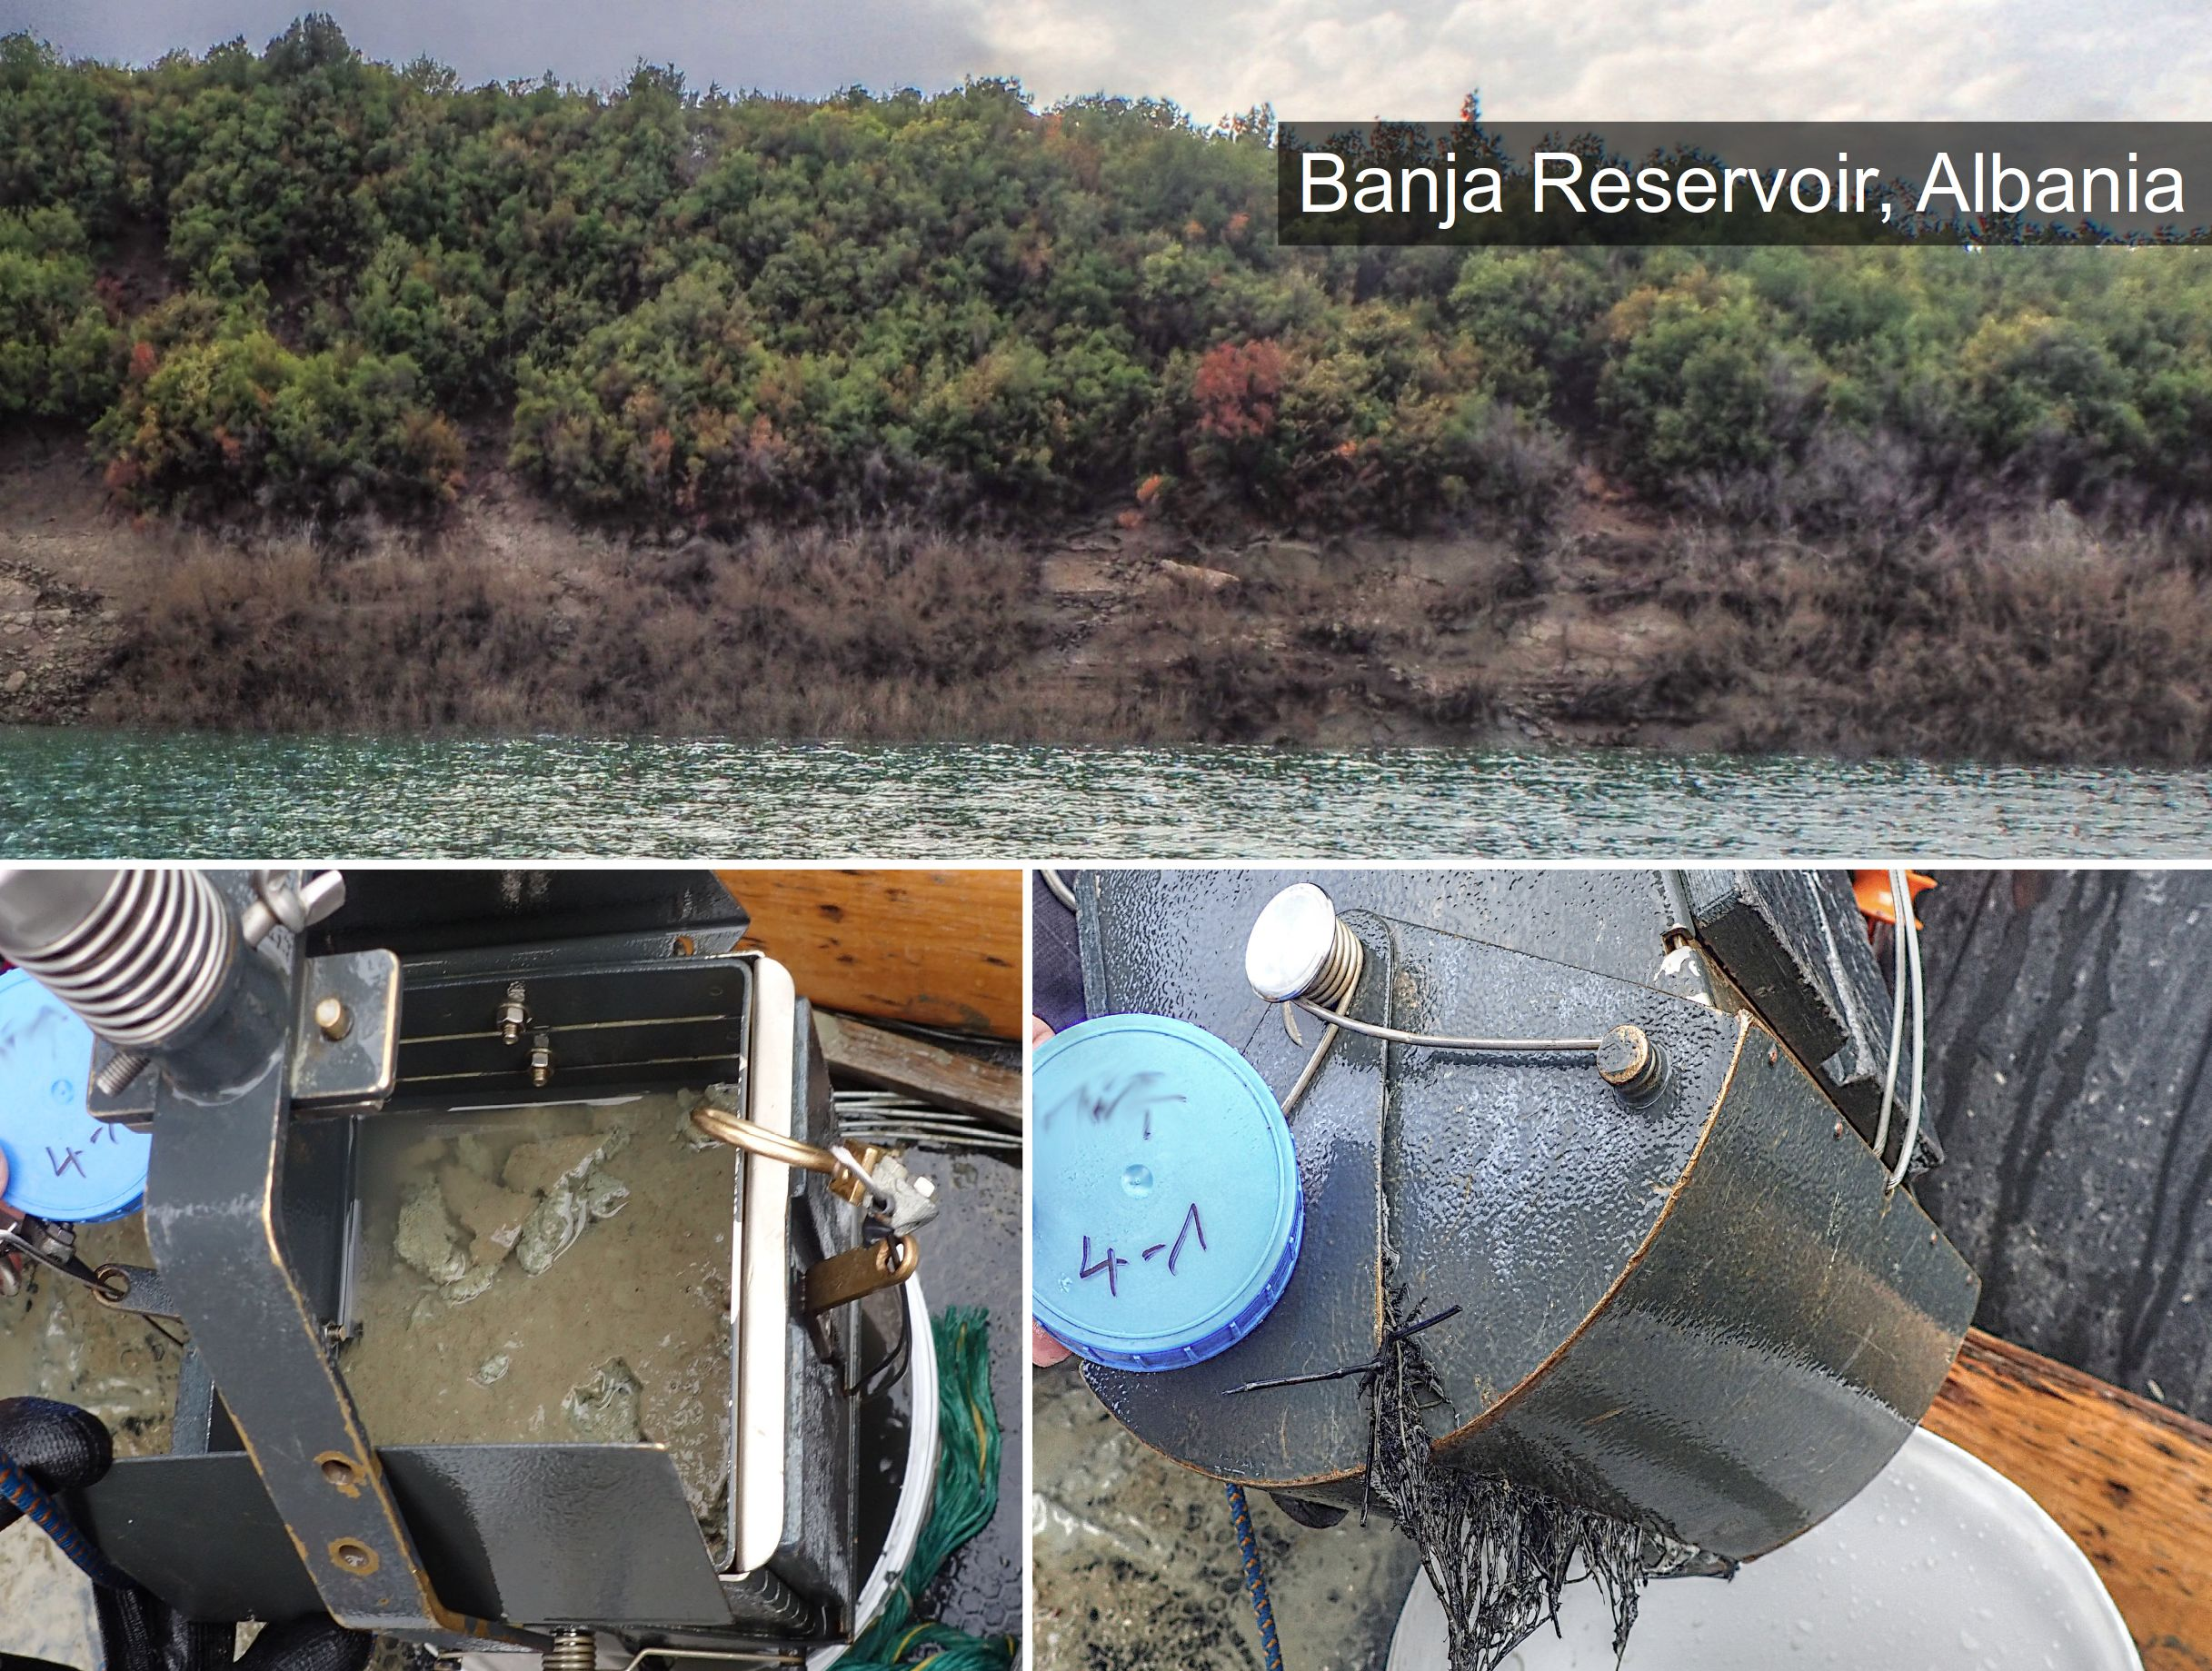
\includegraphics[width=0.73\paperwidth]{banja-mud}};
		\end{scope}}
	\end{tikzpicture}
\end{frame}

\begin{frame}{\secname\vspace{0.1cm}\\\textcolor{anthrazit!80!white}{\subsecname}}
	\begin{tikzpicture}
		\clip (0,0) rectangle (\paperwidth,\paperheight);
		\onslide<1->{
		\begin{scope}
			\node[anchor=south west, xshift=0.05\paperwidth, yshift=0.4\paperheight] {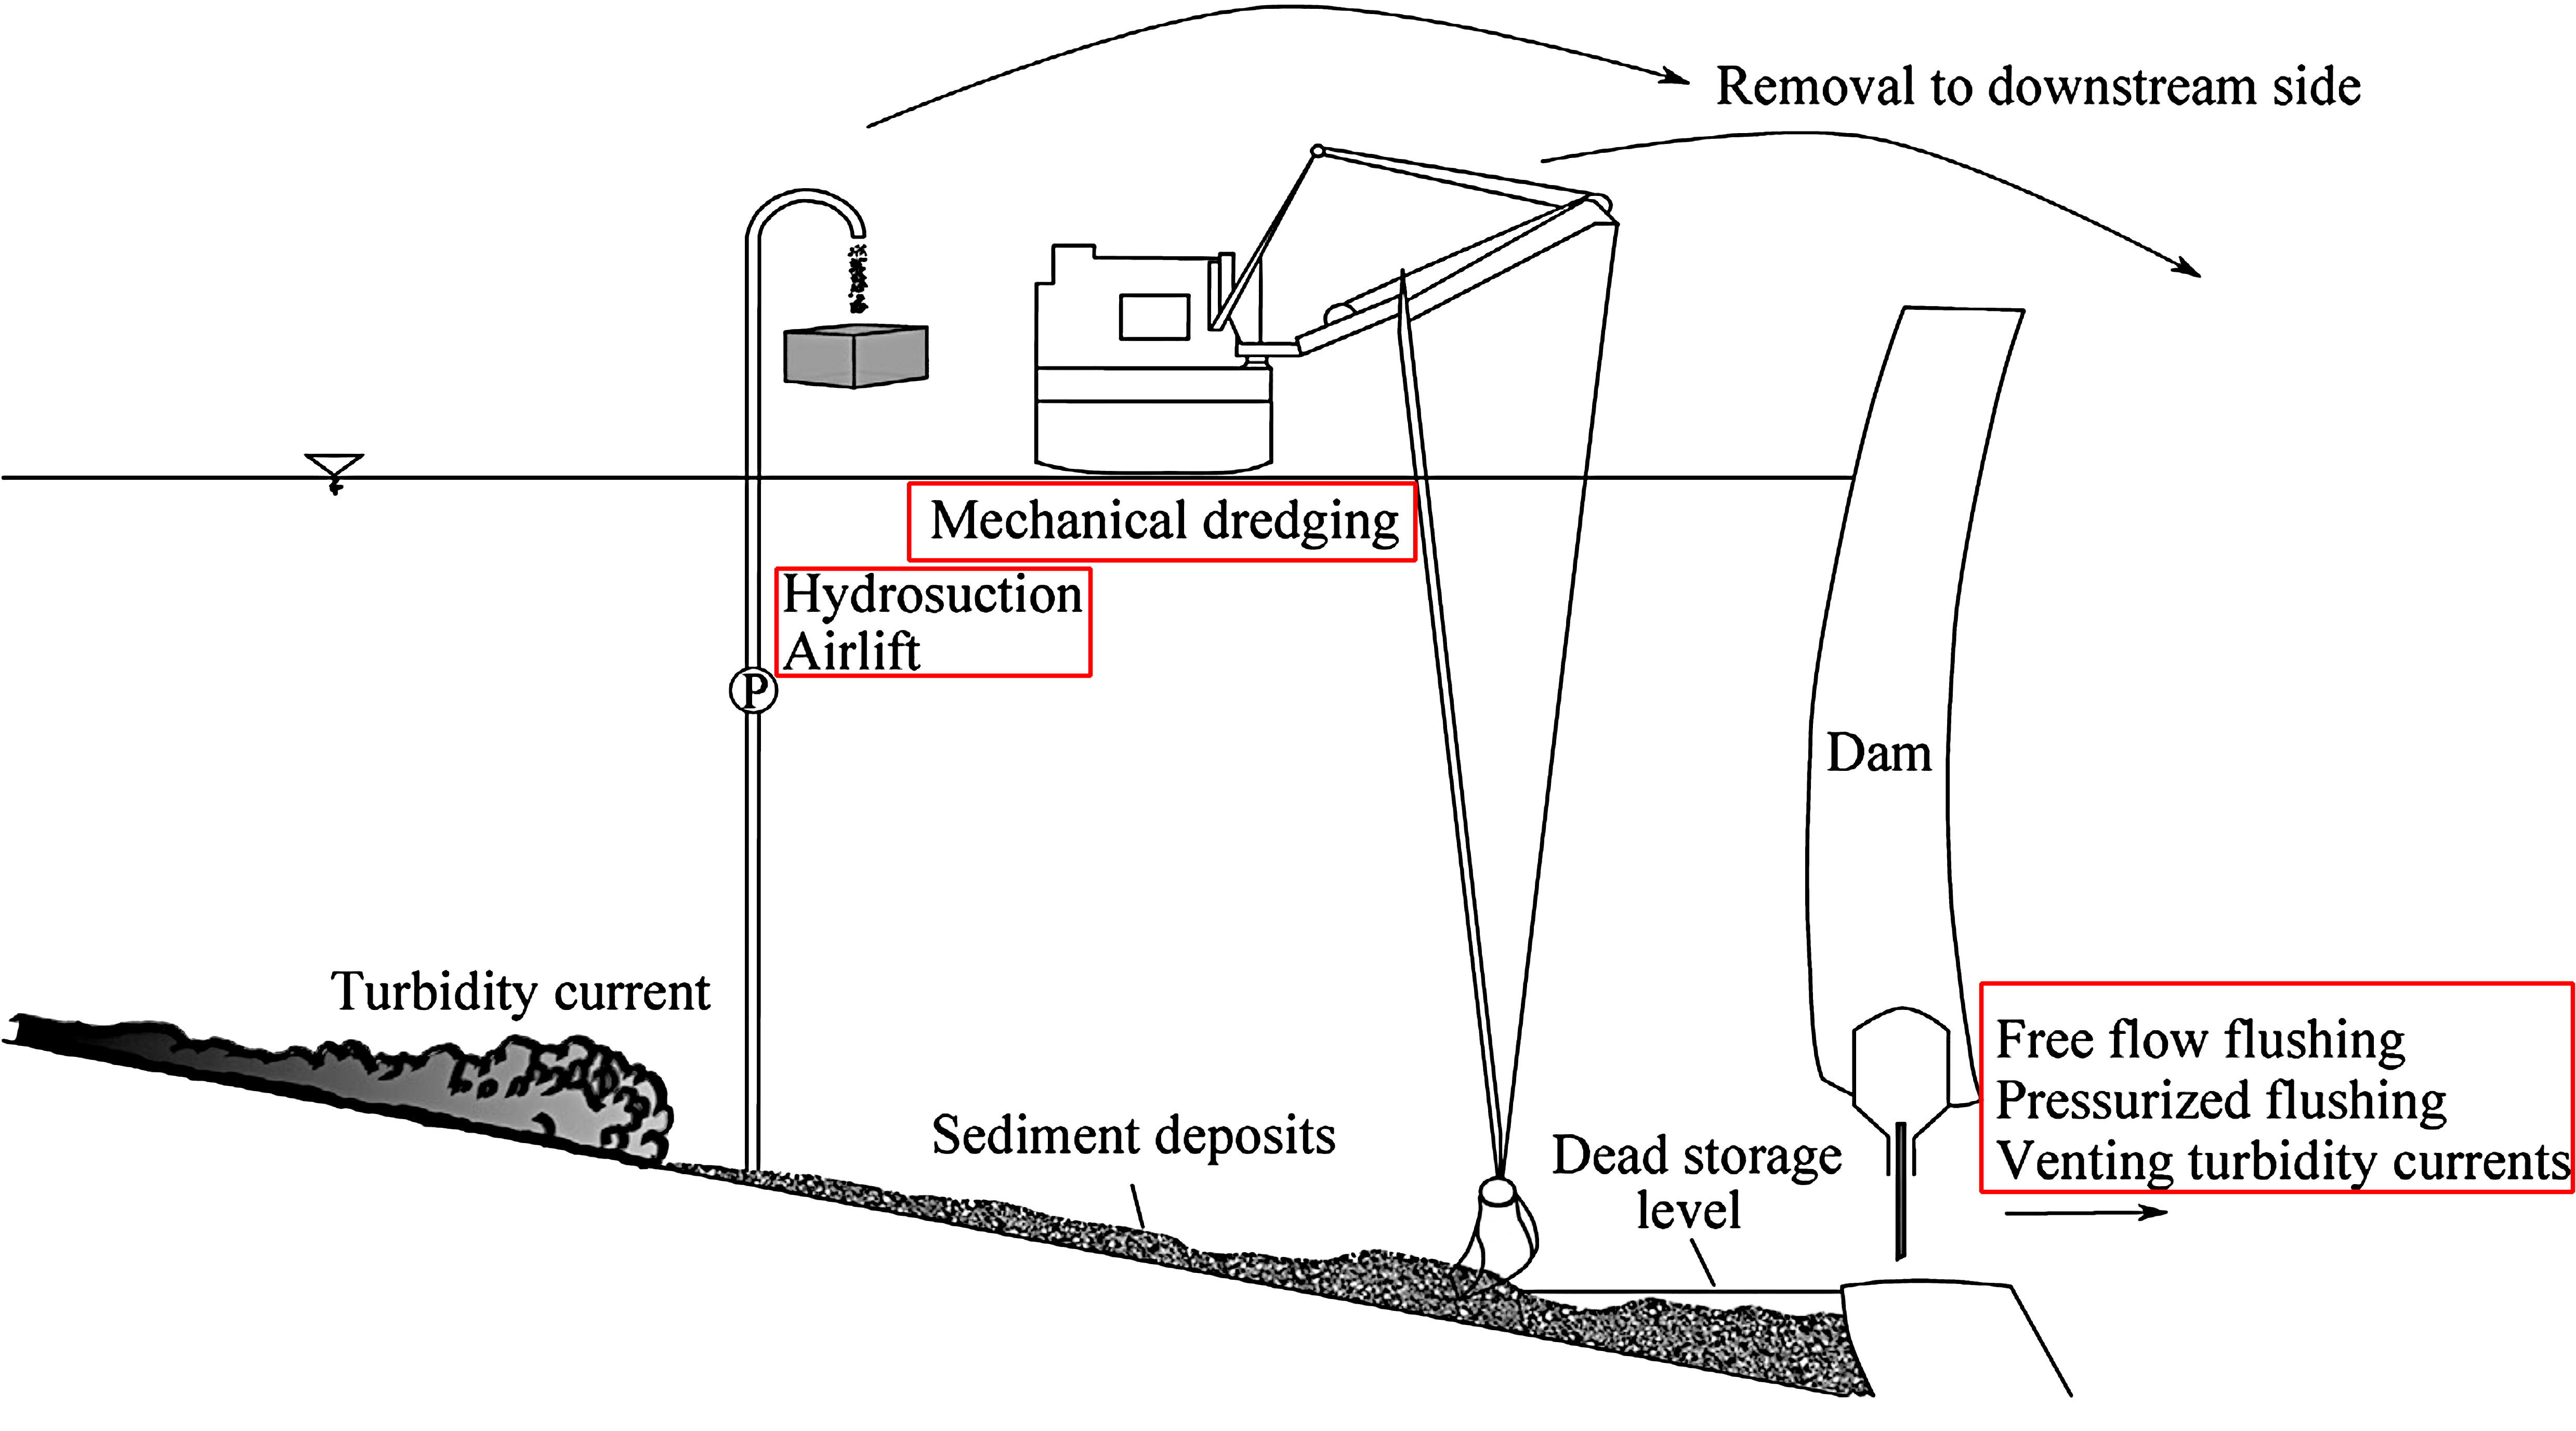
\includegraphics[width=0.78	\paperwidth]{reservoir-sedimentation-mgmt-highlight}};
		\end{scope}}
		\onslide<1->{
		\begin{scope}
			\node[anchor=south west, xshift=0.0\paperwidth, yshift=0.3\paperheight] {
				\begin{minipage}{0.95\textwidth}
					\begin{itemize}
						\item[\faHandORight]\ Airlift / hydrosuction
						\item[\faHandORight]\ Mechanical dredging
						\item[\faHandORight]\ Flushing (free flow, pressurized, venting) \& re-suspension
						\item[\faHandORight]\ Sediment bypass tunnels
					\end{itemize}
				\end{minipage}
			};
		\end{scope}}
		\onslide<1-1>{
			\node[anchor=south west, xshift=0.33\paperwidth, yshift=2.13cm, text=black, text width=0.5\paperwidth,align=left]{\tiny \textcolor{gray}{Source: Chamoun \textit{et al.} / SCCER-SoE (2018)}};}
	\end{tikzpicture}
\end{frame}

\begin{frame}{\secname\vspace{0.1cm}\\\textcolor{anthrazit!80!white}{\subsecname}}
	\begin{center}
		\movie[externalviewer]{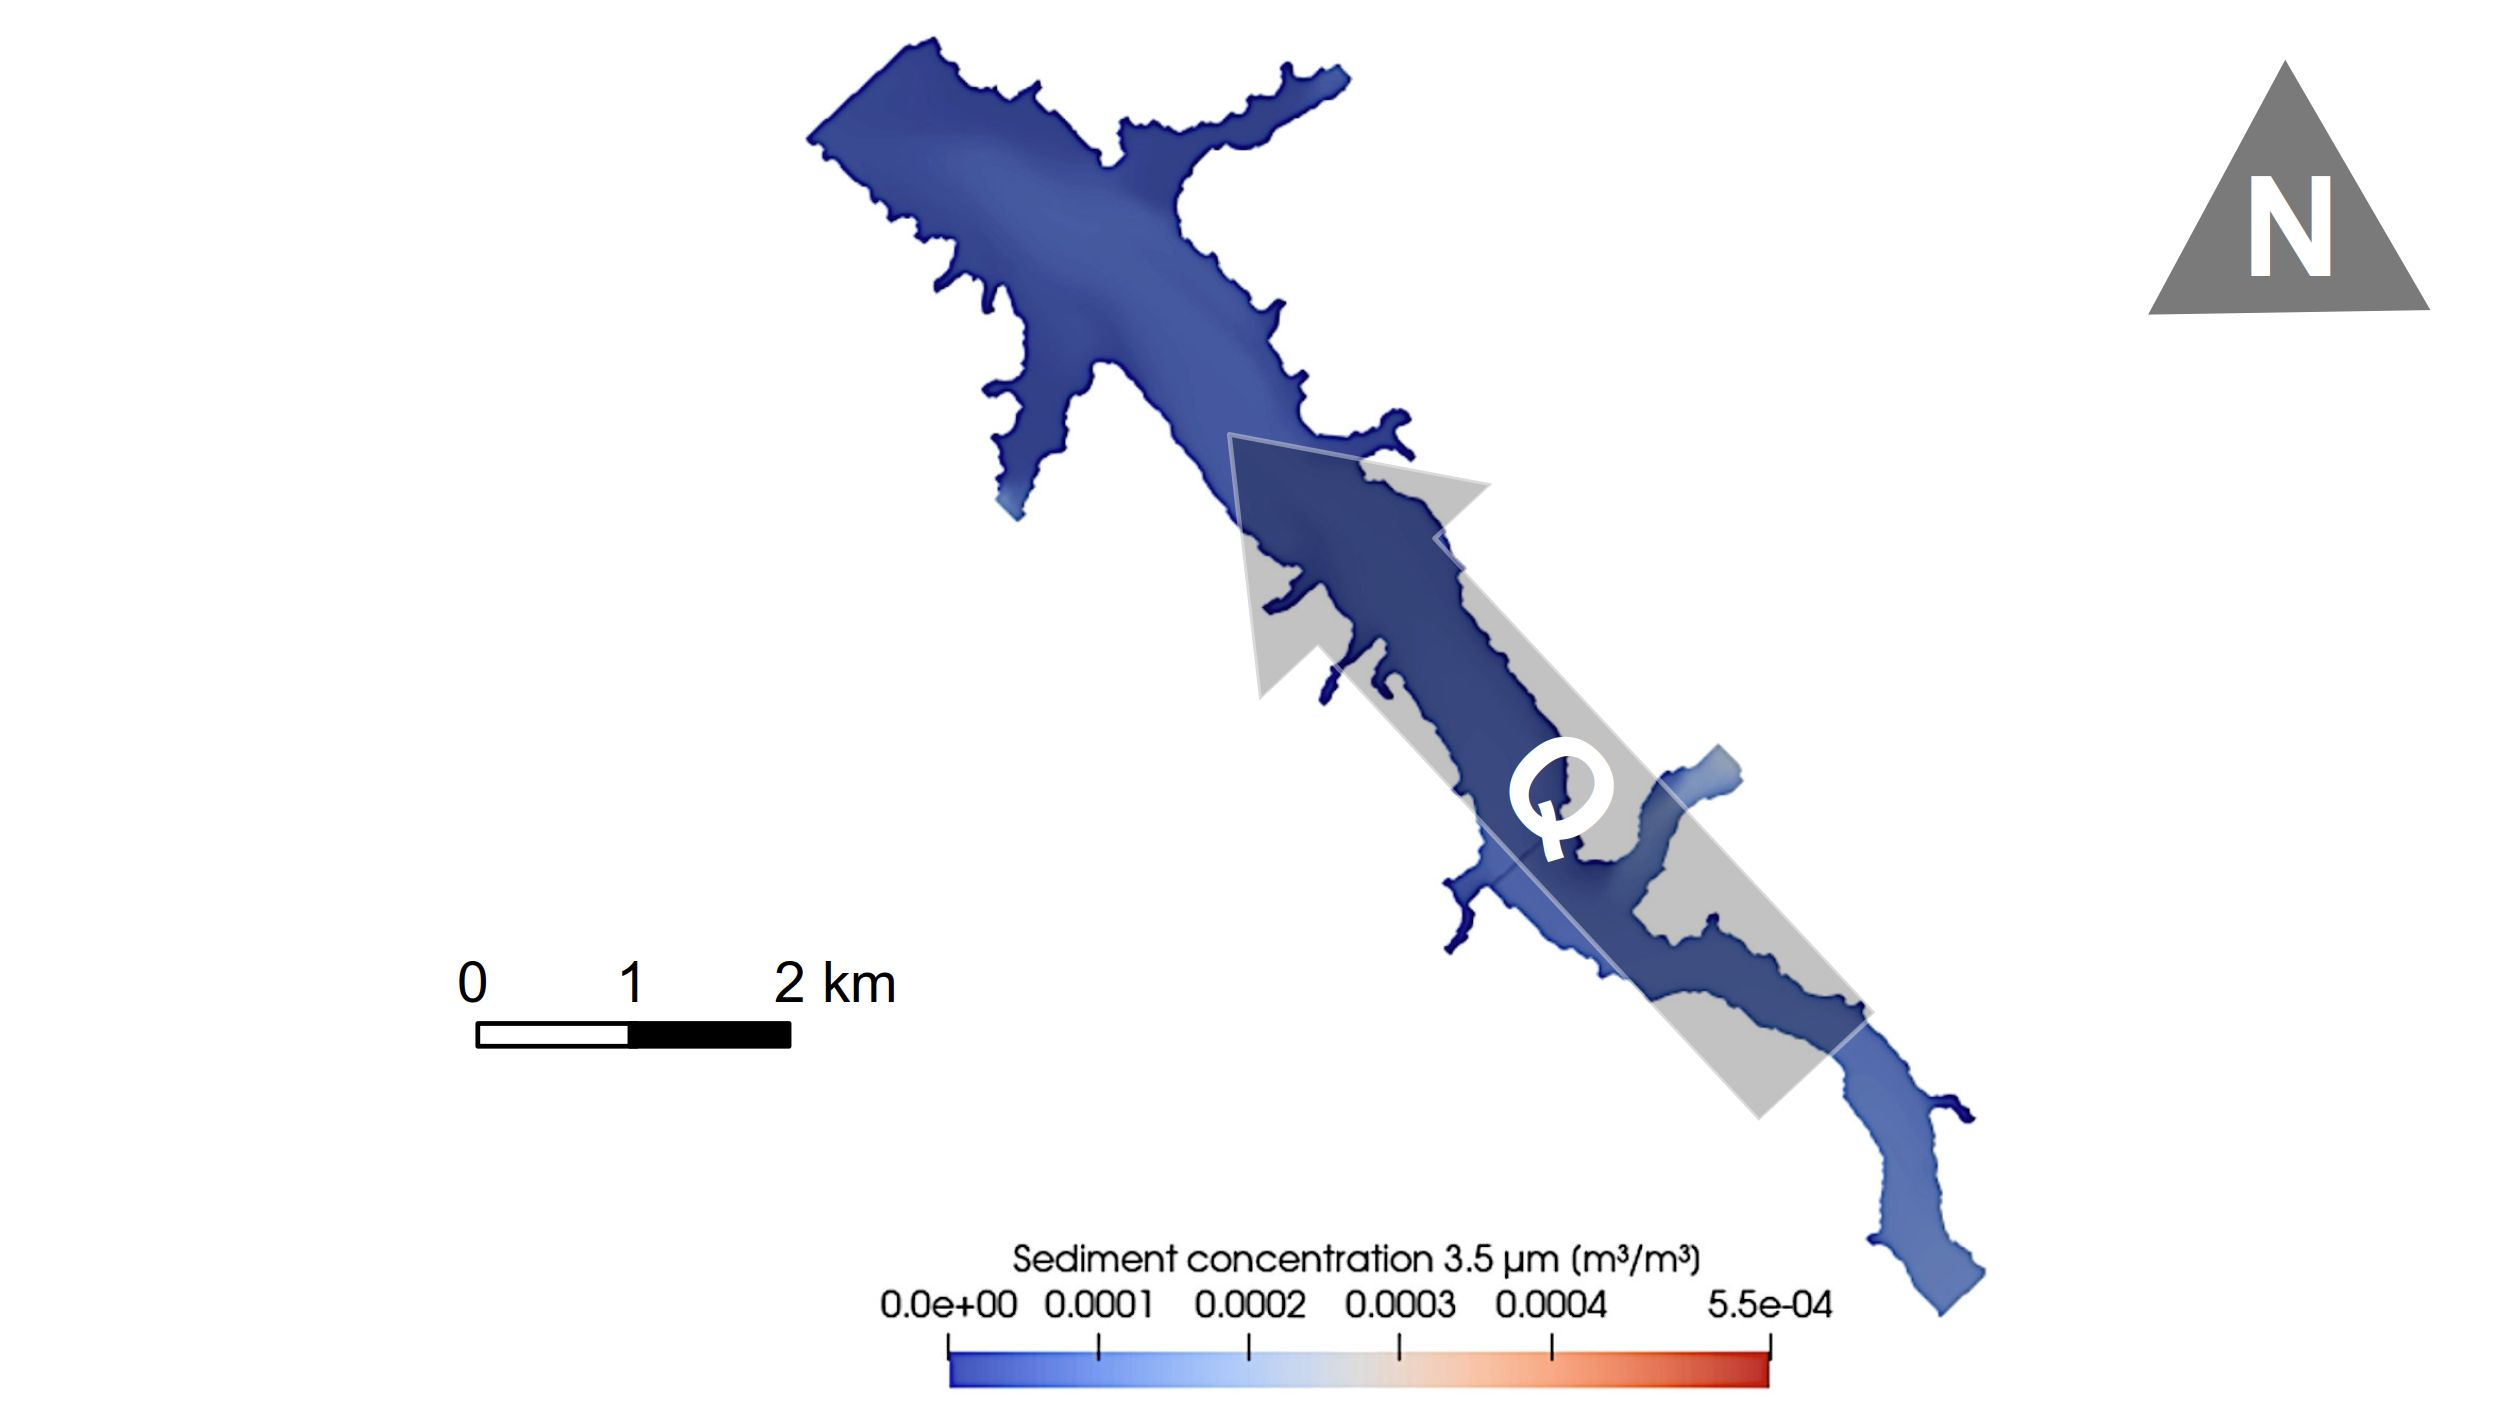
\includegraphics[width=0.95\textwidth,keepaspectratio]{videos/thumbnail-sed-conc.jpg}}{videos/sed-conc.avi}\\
		\textit{Fine particle transport through the Banja reservoir 2016--2019\\
			\textcolor{gray}{(\sscURL{Mouris \textit{et al.}, 2023a}{https://doi.org/10.1007/s40808-023-01712-7}, \sscURL{Mouris \textit{et al.}, 2023b}{https://www.nature.com/articles/s41598-023-47501-1})}}
	\end{center}
\end{frame}
